\documentclass{article}
\usepackage{geometry}
\usepackage{float}
\geometry{letterpaper, margin=1in}
\usepackage{graphicx}
\usepackage[utf8]{inputenc}
\usepackage{listings}
\usepackage{xcolor}
 
\definecolor{codegreen}{rgb}{0,0.6,0}
\definecolor{codegray}{rgb}{0.5,0.5,0.5}
\definecolor{codepurple}{rgb}{0.58,0,0.82}
\definecolor{backcolour}{RGB}{10,22,31}
 
\lstdefinestyle{mystyle}{
    backgroundcolor=\color{backcolour},   
    commentstyle=\color{codegreen},
    keywordstyle=\color{magenta},
    numberstyle=\tiny\color{codegray},
    stringstyle=\color{codepurple},
    basicstyle=\ttfamily\footnotesize\color{white},
    breakatwhitespace=false,         
    breaklines=true,                 
    captionpos=b,                    
    keepspaces=true,                 
    numbers=left,                    
    numbersep=5pt,                  
    showspaces=false,                
    showstringspaces=false,
    showtabs=false,                  
    tabsize=2
}
 
\lstset{style=mystyle}
\title{workspace, package \& publisher}
\author{Student: Alejandro Franco Trujillo Ayala}
\date{\today}

\begin{document}

\maketitle


\section{Introduction}
The present document we use URDF (Unified Robot Description format) this XML file represent a Robot model, we build a Visual Robot Model using editing URDF XML files downloaded from canvas, this code hel

%Resumen, desarrollo, comandos, comprobantes de funcionamiento

\section{Description}

First we neeed to enter our work-space, inside it, we create package with the name urdf\_pkg using the new package:

\begin{figure}[H]
    \centering
    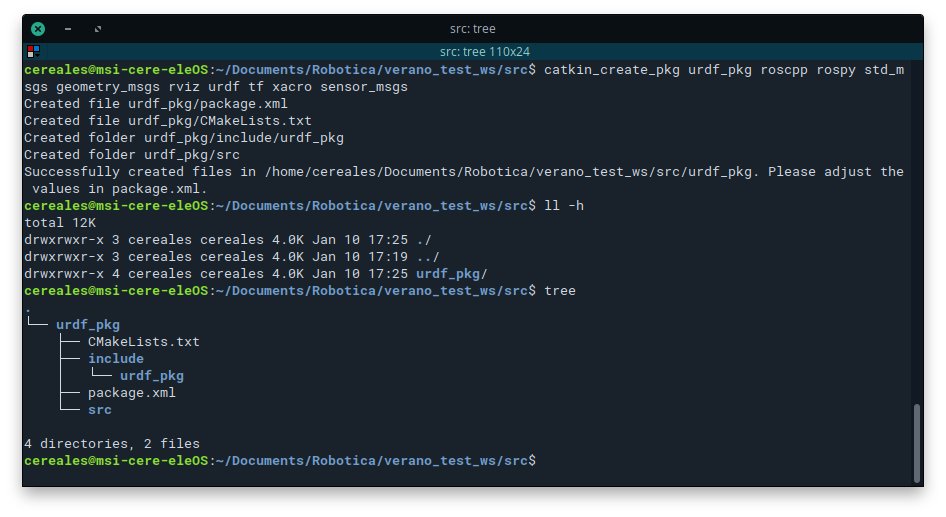
\includegraphics[width=0.9\textwidth]{images/urdf_create.png}
    \caption{creating urdf\_pkg}
    \label{fig:urdf_pkg}
\end{figure}

where:

roscpp = used to compile c++ files to ros\\
rospy = used to compile python files to ros\\
std\_smgs = standard messages to ros with field called "data"\\
geometry\_msgs = provides messages to such as points vectors and poses\\
rviz = 3d visualization environment\\
urdf = it's a analyzer\\
tf = maintains the relationship between coordinate frames in a tree structure buffered in time\\
xacro = XML macros is a macro language you can construct shorter and more readable XML files\\
sensor\_msgs = defines messages to be used sensors\\

Next inside urdf\_pkg we create 2 empty files called : urdf launch
depending to extension file downloaded before we copy one in urdf\_pkg, other in launch and other in urdf

\begin{figure}[H]
    \centering
    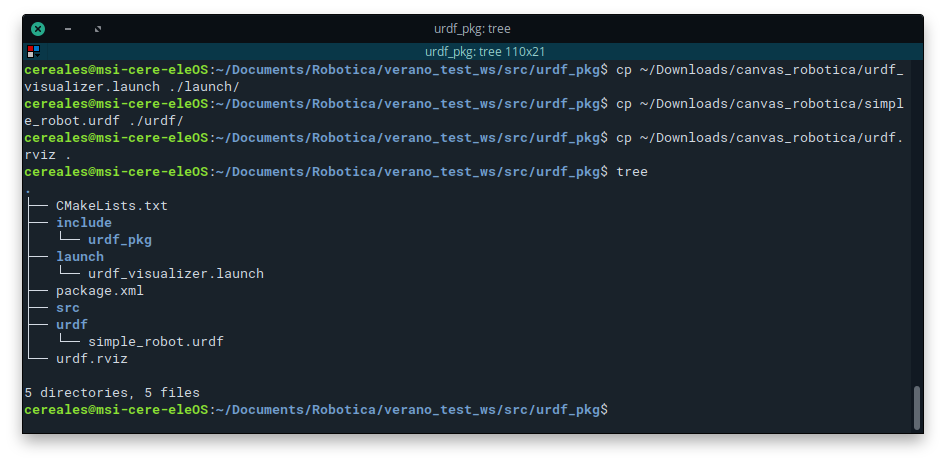
\includegraphics[width=0.9\textwidth]{images/urdf_rviz.png}
    \caption{attaching files inside urdf_pkg}
    \label{fig:urdf_rviz}
\end{figure}

To know if we go in correct steps we launch roslaunch command:




now we realize all change that we want in urdf\_visualizer.launch and 


se realiza cambios en launch y urdf 


creamos 2 archivos launch y urdf

el archivo arviz nos ayuda  a que queremos abrir

roslaunch urd\_pkg urdf\_visualizer.launch

este iforme sera llamado robotics

\section{Commands}

\begin{table}[H]
\begin{tabular}{ll}
\hline
\multicolumn{1}{|l|}{ros cmd} & \multicolumn{1}{l|}{objective}                                    \\ \hline
roscore                           & will start up a ROS master, Parameter server, rosout logging node \\
rosrun basic\_pkg ...     \\         & In the directory basic\_pkg runs the selected code file        \\
rosnode list                      & list active nodes right now                                       \\
rostopic list                     & list active topics                                                \\
rostopic echo ...                 & publish data from selected topic                                  
\end{tabular}
\caption{ROS scripts table used in the report}
\end{table}

\end{document}